\section{Основные интерфейсы}

На предыдущем этапе мы создали вполне работоспособное приложение, но
пользоваться им не удобно и не интуитивно понятно для любого пользователя.
Реализуем интерфейсы редактирования для \verb|Книг| и \verb|Стеллажей|
которые помимо своих собственных сущностей смогут управлять и теми, которые
доступны им по логике применения ИС.

Логически разбобьем всю ИС на две части. Выделим в интерфейс редактирования
стеллажей все что связано с планировкой библиотеки, а также с размещением
книг на стеллажах. Значит нам необходимо работать с сущностями \verb|Зал|,
\verb|Расположение| и непосредственно \verb|Стеллаж|. Во второй интерфейс мы
вынесем оставшиеся сущности связанные с книгами: \verb|Автор|, \verb|Книга|
и \verb|Расположение|.

Для организации интерфейсов мы будем использовать вложенные формы, возможность
использования которых стала доступна при описания нами связей в классах объектов.
Для создания форм связанных моделей используем встроенный метод-хелпер
fields\_for которому передадим форму соответствующей модели созданной
скаффолдом.

Для обеспечения адаптивности, нам необходимо внести в шаблон некоторые
правила каскадных таблиц стилей (CSS), благодаря которым просмотр страницы
будет удобен как на стационарных компьютерах, так и на мобильных устройствах.

Задача адаптивности хоть и совсем непроста, но ее часто необходимо решить.
В условиях подобной необходимости был создан фреймворк Bootstrap.
Это не единственный фреймворк который помогает создать адаптивный
дизайн приложения, но мы будем использовать именно его.

Разобьем наши формы по колонкам используя класс row для контейнера
полей, зададим правила адаптивности колонок и добавим самим полям
класс form-control, тем самым сделаем их более привлекательными.
После этого, в случаем небольшого экрана пользователя, наши формы
будут располагаться в колонку вертикально относительно друг друга.

\begin{small}
\verbatiminput{programms/fields_for.html.haml}
\end{small}

Как можно заметить из примера выше, в шаблоны вложенных форм мы добавим
невидимое поле с идентификатором записи соответствующего объекта. Это
нужно для того, чтобы Ruby on Rails правильно воспринимали получаемые
данные из этих форм: в случае, когда идентификатор не был заполнен,
будет сделана попытка создать новую запись в БД, иначе --- обновить уже
существующую запись в таблице.

Хоть RoR и смогут понять на наличию идентификатора существование сущности
в базе данных, нужно правильно заполнять добавляемые формы на
страницу. Когда создается новый объект поля должны быть изначально
пустыми. А при выборе уже существующего необходимо
заполнять добавленные формы соответствующим им данными.

Поступим следующим образом. Добавив во вложенные формы выпадающий список
с выбором созданных сущностей. При выборе любой из них при помощи JavaScript
мы будем заполнять их данными. Когда же будет выбрано в выпадающем списке
пустое значение (создание новой записи) формы будут очищаться.

Для того, чтобы реализовать задуманное используем технологию AJAX.
AJAX (аббревиатура от «Asynchronous Javascript And Xml») – технология
обращения к серверу без перезагрузки страницы. За счет этого
уменьшается время отклика и веб-приложение по
интерактивности больше напоминает десктоп.

Несмотря на то, что в названии технологии присутствует буква X
(от слова XML), использовать XML вовсе не обязательно.
В мире сложилось так, что часто под AJAX подразумевают также
любое общение с сервером без перезагрузки
страницы, организованное при помощи JavaScript. Хотя в формально
не все такие запросы считаются ajax-запросами.

Создадим отдельный экшен, который будет возвращать ответ клиенту в
формате \texttt{js}, так не будет происходить перезагрузки страницы.

В папке представлений создадим файл с coffee-скриптом имеющий название
соответствующиего ему экшена. Именно этот скрипт
будет исполнен в ответ за запрос
с клиентской части.
Поручим ему очистку и заполнение форм
в зависимости от реакции контроллера.

Осталось добавить ajax-запрос при самом изменении выпадющего списка.
В папке \texttt{javascript} откроем файл общих скриптов для
страниц нашего интерфейса и при помощи библиотеки jQuery
создадим обработчик события изменения выпадющего списка,
который будет отправлять в контроллер выбранное значение
по схеме AJAX. В случае интерфейса книг такой обработчик
может быть написан так:
\begin{small}
\verbatiminput{programms/fill_nested_fields.coffee}
\end{small}
\noindent
Помимо выбранного значения отправляется также уникальный фрагмент имени
самой формы в DOM-структуре страницы по которому конечный скрипт
будет определять точную форму для заполнения данными.

Используем метод гема cocoon для ссылки добавления и удаления
самой вложенной формы на
страничку; использование этого гема сильно
облегчает нашу работу, ведь
с ним нам не нужно самим писать код для создания кнопки добавления форм и
заботиться о том, чтобы rails смогло корректно обработать их,
также не нужно будет организовывать методы удаления связей между объектами.

Для улучшения внешнего вида добавим несколько правил оформления стилей.
В результате форма редактирования книги имеет такой вид:
\begin{figure}[ht!]
\begin{center}
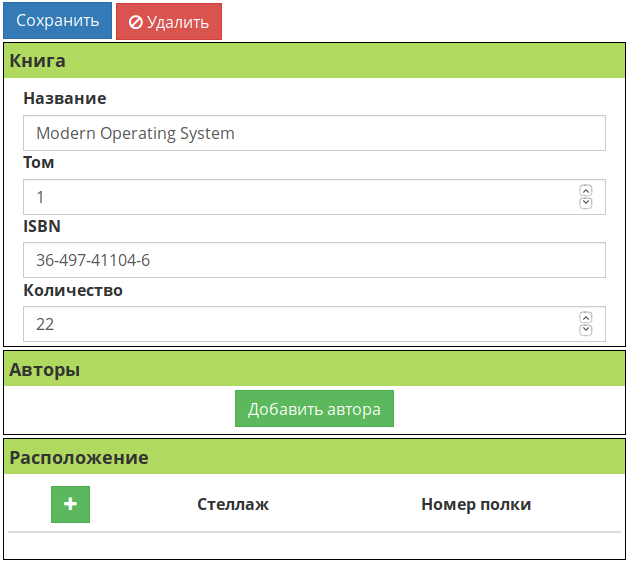
\includegraphics[scale=0.75]{images/book-form2.png}
\end{center}
\vspace*{-8mm}
\caption{Форма редактирования книги} \label{fig:book-form2}
\end{figure}

Закончив с настройкой вложенных форм можно перейти к оформлению списков
книг и стеллажей. Необходимо сделать так, чтобы в описании одной сущности
была вся информация о ней, а так же о сущностях которые ей доступны.

Будем применять относительно новую технологию в CSS именуемой flex-box.
Контейнеры с его свойствами будут менять исходя из размеров экрана.
Подобные технологии получили название Отывчивых (Responsive) и их
главное отличие от Адаптивных (Adaptive) в том, что они не используют
медиа-запросы и не привязываются к конкретным значениям ширины и высоты.
Две эти технологии направлены на решение одной задачи и выбор использования
одной из них - дело вкуса и предпочтений. В руках умелого верстальщика
оба этих инструмента могут использоваться в одном проекте.

Создав подобные списки можно заняться их внешним видом более детально.
Украсим их стандартными css-правилами и корректно переведем все
необходимые строки на русский язык. Добавим навигацию в верхнюю
часть страницы в виде «хлебных крошек» (breadcrumbs) с помощью
которой пользователь без труда будет ориентироваться
в структуре приложения.

Навигационная цепочка
«Хлебных крошек» --- элемент навигации
по веб-сайту, представляющий собой путь по сайту от
его «корня» до текущей страницы, на которой находится пользователь.

Название «Хлебные крошки» является иронической отсылкой к
немецкой сказке «Гензель и Гретель», в которой дети,
когда их завели в лес во второй раз, не смогли найти
обратную дорогу, так как на этот раз вместо маленьких камешков они
оставляли за собой хлебные крошки, впоследствии склёванные лесными птицами.

Существует огромное множество реализаций подобных систем навигации.
Их число определяется тем, что вместе с прикладной значимостью
«хлебные крошки» --- элемент дизайна сайта, который может подстраиваться
под окружения любого приложения. В нашем случае мы построим
такую цепочку просто разделив ее элементы символом-стрелочкой.

%\newpage
Конечный результат для списка \verb|Стеллажей| можно видеть на
следующем изображении:

\begin{figure}[ht!]
\begin{center}
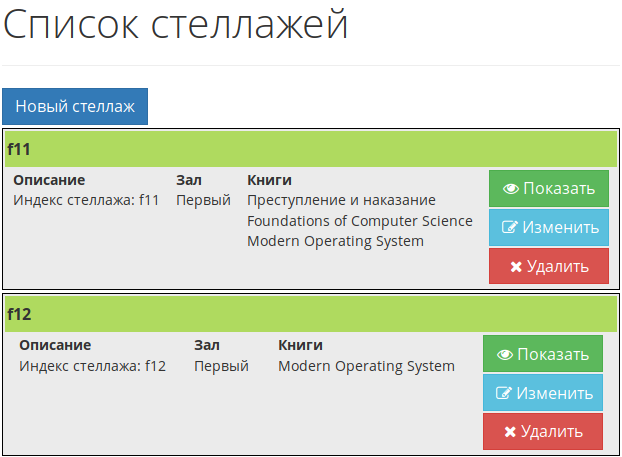
\includegraphics[scale=0.75]{images/shelves-index.png}
\end{center}
\vspace*{-8mm}
\caption{Список стеллажей} \label{fig:shelves-index}
\end{figure}

Разделение ответственностей и обязанностей между ролями тоже
входит в задачи нашей информационной системы. Допустим, что
необходимо допустить всего две основные роли: администратор и оператор.

Обозначим доступные им возможности ИС. В случае администратора все
банально и просто - он может все (подобную роль необходимо назначать
пользователям с осторожностью, ведь у них будет полный доступ к приложению!).
Оператору мы позволим использовать возможности интерфейсов редактирования
\verb|Книг| и \verb|Стеллажей| в полной мере, но полностью запретим
ему доступ к части администрирования. Незарегистрированному пользователю
позволим просматривать списки стеллажей и книг.

В Rails подобные ограничения необходимо выполнить в виде
методов-фильтров, которые будут запускаться перед или после
определенными экшенами
контроллера. Разместить их необходимо разумеется в них.

\newpage

Чтобы не загромождать модели определениями каждой из необходимых нам
функций, мы будем использовать возможности объекта Proc (создадим его потомка
lambda для лямбда-функций) определяя права текущего пользователя. Контроллер
для \verb|Книг| преобразуется следующим образом:

\begin{small}
\verbatiminput{programms/book_controller.rb}
\end{small}

Добавленная лямбда-функция в классе контроллера находится на третей строчке
и ее начало обозначается стрелочкой. На предыдущих строках
описан фильтр позволяющий просматривать списки книг и описание отдельных
экземпляров. Сам этот метод реализован в базовой версии проекта
и поэтому рассматриваться нами не будет.

На данном этапе приложение включает в себя адаптивно реализованные
интерфейсы для \verb|Книг| и \verb|Стеллажей| с вложенными
формами. Настроена система навигации
и авторизации. Проект полностью русифицирован.
